

\documentclass{article}
\usepackage[utf8]{inputenc}
\usepackage{setspace}
\usepackage{ mathrsfs }
\usepackage{graphicx}
\usepackage{amssymb} %maths
\usepackage{amsmath} %maths
\usepackage[margin=0.2in]{geometry}
\usepackage{graphicx}
\usepackage{ulem}
\setlength{\parindent}{0pt}
\setlength{\parskip}{10pt}
\usepackage{hyperref}
\usepackage[autostyle]{csquotes}

\usepackage{cancel}
\renewcommand{\i}{\textit}
\renewcommand{\b}{\textbf}
\newcommand{\q}{\enquote}
%\vskip1.0in





\begin{document}

{\setstretch{0.0}{
Loop [ Julia Version ]

Loop is a relatively simple symmetric cryptosystem. The key is a permutation of $\{k \in \Bbb N \ | \  1 \le k \le n \}$. This permutation is written in the abbreviated form  of $f = f(1)f(2)...f(n)$. For instance, if $n = 4$, then one such key would be $f = 2314$, with $f(1) =2, f(2) = 3, f(3) = 1, f(4) = 4$. 

An adjustable \q{alphabetic mask} is also used for a more human-readable output. For instance, we can set $n = 26$ and then translate representations of the key, plaintexts, and ciphertexts by $1 \to a, 2 \to b,3 \to c,...$. The image below shows output from the demo function. First the key is given, then the number of rounds of encryption. Finally the key (more exactly a function parameterized by the key) is applied to various random permutations. 
\begin{figure}[h!]
\end{figure}

%\begin{figure}
%  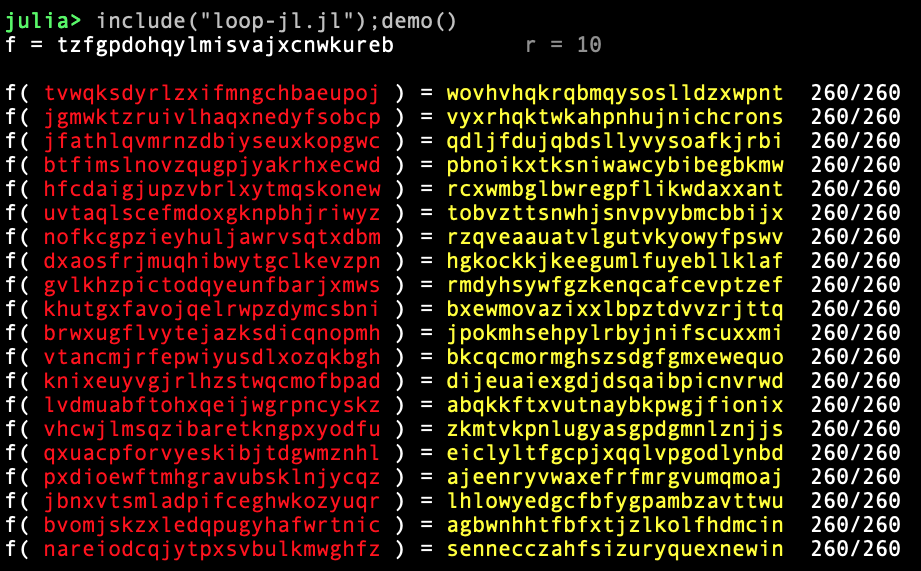
\includegraphics[width=\linewidth]{ex.png}
%  \caption{}
%  \label{}
%\end{figure}

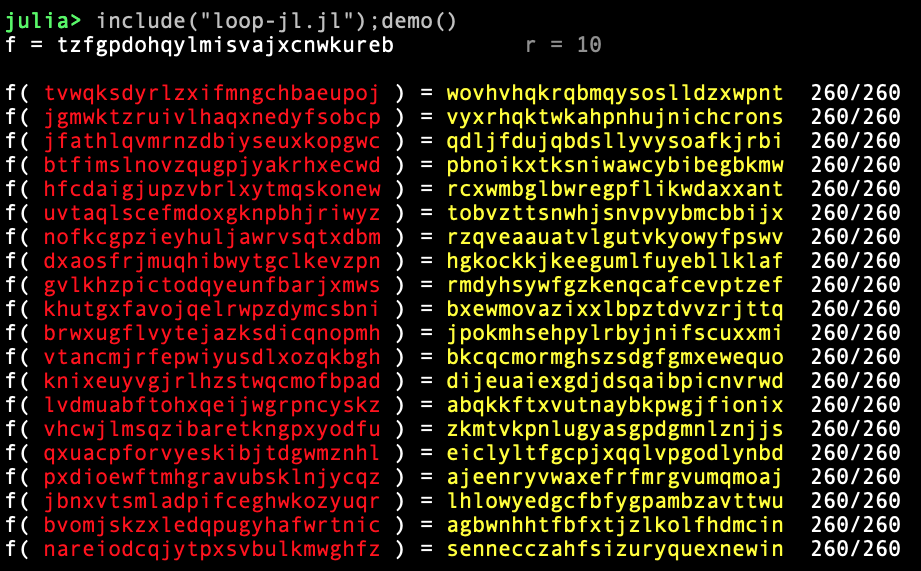
\includegraphics[width=0.5\textwidth]{ex.png}


The fraction that follows each $f(p) = c$ is the count of unique permutations over the number of symbols processed. The set $F$ accumulates keystates, which are counted later. After a symbol of plaintext is processed, the key $f$ is transformed in a way that depends on that plaintext symbol and its own current state. In particular, $g$ is computed as the circular shift of $f$ by $p$ positions. Then we get $f' = g \circ f$, where $f'$ is the new keystate. Here's the process expressed in the code:

\begin{verbatim}
function encode(p,q,F)
    f = copy(q)
    c = Int64[]
    for i in eachindex(p)
        push!(c,f[p[i]])
        g = circshift(f,p[i])
        f = comp(g,f)
        push!(F,f)
    end
    c
end

\end{verbatim}

Ideally, key states are not repeated, and $f'$ is a brand new permutation unseen till now, but this ideal depends on $n$ being sufficiently large. A value of $n = 26$ almost always leads to consistently unique keystates ( at least up to 100 rounds.) Note that there are $26! = 403291461126605635584000000$ possible keys, at least for $n =26$, so Loop \i{might} be reasonably secure. It is offered though more as a toy or a sculpture than as a serious security tool.  



}}
\end{document}
